\documentclass{beamer}
\usetheme{Madrid} % My favorite!
\setbeamercovered{invisible}
\usefonttheme{serif}
% To remove the navigation symbols from 
% the bottom of slides%
\setbeamertemplate{navigation symbols}{} 
% 
\usepackage{graphicx}
% 
\title[Online Social Network Privacy]{A Framework for Computing the
  Privacy Scores of Users in Online Social Networks}
\author{Kun Liu}

\date{\today}
\begin{document}
% Title page of this presentation. 
\begin{frame}
  \titlepage
\end{frame}

% problem and contribution. 
\begin{frame}
  \frametitle{Problem Description}
  \begin{block}
    {How to measure privacy risk of social network users?}
    \begin{itemize}
      \LARGE{
    \item Privacy protection Related works. 
      \begin{itemize}
        \Large{
      \item Spamming and Phishing.
      \item Social network Attacks. 
      \item Access control privacy control.
      \item Multi-party collaborative privacy control. 
      \item ...}
      \end{itemize}
    \item What is the privacy risk level? }
    \end{itemize}
  \end{block}
\end{frame}

% Contribution of this paper.
\begin{frame}
  \frametitle{Contributions of This Paper}
    \begin{itemize} 
      \LARGE{
      \item A privacy score computation model. 
      \item Model validation method. }
    \end{itemize}
\end{frame}

\begin{frame}%[fragile] % Notice the [fragile] option %
  \frametitle{General Observations and Intuitions}
  \begin{itemize}
    \item Different profile items(e.g. name, age, address etc.) can
      contribute differently to the privacy score calculation. \\
      - We call this difference sensitivity. \\
      - This property usually depends on the item itself. E.g. some
      items are inherently more sensitive than others. 
    \item It is common that the more people who can see user's online
      information, the higher risk user will have. Thus, we can use
      the scope of information visibility as a factor for privacy
      score calculation. \\
      - We call this factor visibility in the privacy score model. 
  \end{itemize}
\end{frame}

% Modelling online social network profile settings. 
\begin{frame}[fragile]
  \frametitle{Modeling Social Network Users}

  \begin{figure}
    \begin{center}
      
\includegraphics[scale=1.5]{socialnetwork}
    \end{center}
  \end{figure}

\[
\Longrightarrow
 R_{n,N} =
 \begin{pmatrix}
  R_{1,1} & R_{1,2} & \cdots & R_{1,N} \\
  R_{2,1} & R_{2,2} & \cdots & R_{2,N} \\
  \vdots  & \vdots  & \ddots & \vdots  \\
  R_{n,1} & R_{n,2} & \cdots & R_{n,N}
 \end{pmatrix}
\]

\end{frame}

% IRT model description.
\begin{frame}[fragile]
  \frametitle{The Item Response Theory(IRT) Model}
  \[\LARGE{P_{ij}=\frac{1}{1+e^{-\alpha_i(\theta_j-\beta_i)}}}\]
\end{frame}

% IRT based Privacy score model. 
\begin{frame}
  \frametitle{IRT based Privacy Score model.}
  We can use IRT to model the privacy score estimation. But we need to
  reinterpret the IRT model as follows. \\ 
  \begin{enumerate}
    \item Examinee mapped to a user and question mapped to profile
      item. 
    \item The ability of examinee $\theta_j$ corresponses to attitude of
      user $j$. 
    \item The difficulty $\beta_i$ corresponses to
      \textit{sensitivity} of of profile item $i$. 
    \item Question discrimination parameter $\alpha_i$ is ignored, and
      it can be used to adjust the analysis of items and users. 
  \end{enumerate}
\end{frame}

% privacy score definition.
\begin{frame}[fragile]
  \frametitle{Definition of the Privacy Score}
  Intuitively, the privacy score should be monotonically increasing with
  both sensitivity and visibility. So, this paper defines privacy
  score of user $j$ for item $i$ as \textsc{Pr}$(i,j)=\beta_i\times
  V(i,j)$, and by summing up all the item privacy for user $j$, we get
  the privacy score for user $j$ as
  \[\textsc{Pr}(j)=\sum_{i=1}^{n}\textsc{Pr}(i,j)=\sum_{i=1}^n\beta_i\times V(i,j). \]
 In this definition, $V(i,j)$ represents the visibility of item $i$
 for user $j$, and it can be calculated by
   \[V(i,j)=P_{ij}\times 1 + (1-P_{ij})\times 0 = P_{ij}\]
   where \[P_{ij} = Prob\{\textbf{R}(i,j)=1\}.\]
 So, in order to calculate the privacy score $\textsc{Pr}(j)$, we need
 to estimate sensitivity $\beta_i$ and visibility $V(i,j)$.
\end{frame}

% Estimating sensitivity with MLE. 
\begin{frame}
  \frametitle{\large{Estimating sensitivity $\xi_i=(\alpha_i,\beta_i)$ when
      $\overrightarrow{\theta}=(\theta_1,\dots,\theta_N)$ is known.}}
  \begin{block}
      {Use Maximum Likelihood Estimation(MLE).}
      \[\xi_i^{MLE}=\underset{\xi}{\operatorname{\arg\max}}
      {\prod_{j=1}^NP_{ij}^{R(i,j)}(1-P_{ij})^{1-R(i,j)}}\]
      Partition social network users $\{1,\dots,N\}$ into $K$
      non-overlapping groups $\{F_1,\ldots,F_K\}$ s.t. $\cup_{g=1}^KF_g=\{1,\ldots,N\}$. \\ 
      We can derive log-likelihood function as : 
      \[\xi_i^{MLE}=\underset{\xi}{\operatorname{\arg\max}}
      {\sum_{g=1}^K[r_{ig}logP_i(\theta_g)+(f_g-r_{ig})log(1-P_i(\theta_g))]}\]
      $K$ is the total number of groups; \\
      $r_{ig}$ is the number of users in group $g$ who set item $i$ to one; \\
      $\theta_g$ is the attitude of group $g$ and \\
      $f_g=|F_g|$ is total number of users within group $F_g$.
  \end{block}
\end{frame}

% Estimating sensitivity with EM method.
\begin{frame}
  \frametitle{\small{Estimating sensitivity $\xi_i=(\alpha_i,\beta_i)$ when
      $\overrightarrow{\theta}=(\theta_1,\dots,\theta_N)$ is unknown.}}
  \begin{block}
      {Use Expectation Maximization (EM) method.}
      \textbf{E-Step:} compute $E[f_g]$ and $E[r_{ig}]$ as follows:
      \[E[f_g]=\overline{f_g}=\sum_{j=1}^NP(\theta_g|R^j,\overrightarrow{\xi})\] 
      \[E[r_{ig}]=\overline{r_{ig}}=\sum_{j=1}^NP(\theta_g|R^j,\overrightarrow{\xi}\times R(i,j)).\]
      $P(\theta_g|R^j,\overrightarrow{\xi})$ denote the posterior probability
      distribution of a user's attitude. 

      \textbf{M-Step:}
      With the values of $\overline{f_g}$ and $\overline{r_{ig}}$, we can
      compute a new estimate of $\overrightarrow{\xi}$ with the Newtown-Raphson
      item-parameters estimation procedure. 
  \end{block}
\end{frame}

% posterior probability calculation. 
\begin{frame}
  \frametitle{Calculating the Posterior Probability of Attitudes}
  \[P(\theta_j|R^j,\overrightarrow{\xi})=\frac{P(R^j|\theta_j,\overrightarrow{\xi})g(\theta_j)}
  {\int{P(R^j|\theta_j,\overrightarrow{\xi})g(\theta_j)d\theta_j}}\]
  By partitioning user attitude into different groups, we can transform the $\int$
  to $\sum$ as show below: 
  \[P(\theta_j|R^j,\overrightarrow{\xi})=\frac{P(R^j|X_t,\overrightarrow{\xi})g(X_t)}
  {\sum_{t=1}^K{P(R^j|X_t,\overrightarrow{\xi})g(X_t)}}\]
  In this formula, $K$ is the number of groups of user attitudes, and user
  attitudes are partitioned into points $\{X_1,X_2,\ldots,X_K\}$. $A(X_t)$ is
  the attribute probability value determined by $X_t$ and $\sum_{t=1}^KA(X_t)=1$.
\end{frame}

% 
\begin{frame}
  \frametitle{IRT-Based Computation of visibility}
  {$V(i,j)=P_{ij}=Prob\{R(i,j)=1\}$}
  \begin{itemize}
  \item If $\overrightarrow{\theta}, \overrightarrow{\alpha},
    \overrightarrow{\beta}$. Visibility can be calculated using IRT
    probability formula. 
  \item If parameters are not given, they can be estimated using MLE/EM method,
    and similarly, $\overrightarrow{\theta}$ can be estimated with MLE method
    as follows: 
    \[\overrightarrow{\theta^{MLE}}=\underset{\xi}{\operatorname{\arg\max}}
      {\sum_{i=1}^n[R(i,j)logP_{ij}+(1-R(i,j))log(1-P_{ij})]}\]
    \end{itemize}
\end{frame}

\begin{frame}
  \frametitle{Polytomous Privacy score computation}
  The above dichotomous privacy model can be easily promoted to the one with
  multiple privacy settings. (Omitted currently)
\end{frame}

% 
\begin{frame}
  %\frametitle{Finally, we can compute the privacy score use IRT method}
  \frametitle{A naive privacy score computation method}

  \textbf{Naive computation of Sensitivity:}
  \[\beta_i=\frac{N-|R_i|}{N}\] 
  $|R_i|$ is the number of users who set item $i$ as visible. or 
  \[\beta_{ik}^*=\frac{N-\sum_{j=1}^NI_{R(i,j)\leq k}}{N}\] for polychotomous case. 

  \textbf{Naive computation of Visibility:}
  \[P_{ij}=\frac{|R_i|}{N}\times \frac{|R^j|}{n}\] and 
  \[P_{ijk}=\frac{\sum_{j=1}^NI_{(R(i,j)=k)}}{N}\times
  \frac{\sum_{i=1}^nI_{R(i,j)=k}}{n}\]
  for polychotomous case. 
\end{frame}

\begin{frame}
  \frametitle{Experiment results}
  \begin{figure}
    \begin{center}
    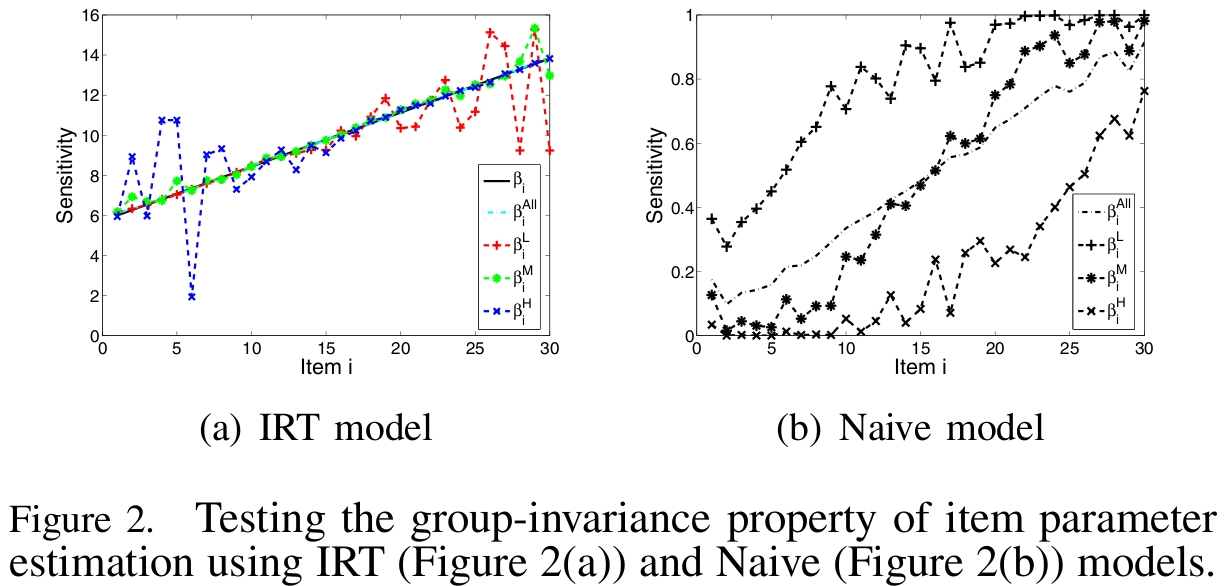
\includegraphics[scale=0.25]{result}
  \end{center}
  \end{figure}
\end{frame}

\begin{frame}
  \frametitle{Weakness of this paper}
  \begin{enumerate}
    \item This paper fails to explicitely consider the effects of
      social graph. 
    \item This paper doesn't consider the balance between privacy and
      utility. Utility here is not clearly defined. 
  \end{enumerate} 
\end{frame}

\begin{frame}
  \centerline{The End, Thanks!}
\end{frame}
% End of slides
\end{document}